\subsection{Tan\-Pix2Ra\-Dec  Class Reference}
\label{class_tanpix2radec}\index{TanPix2RaDec@{Tan\-Pix2Ra\-Dec}}
the transformation that handles pix to sideral transfos (Gnomonic, possibly with polynomial distortions). 


{\tt \#include $<$gtransfo.h$>$}

Inheritance diagram for Tan\-Pix2Ra\-Dec::\begin{figure}[H]
\begin{center}
\leavevmode
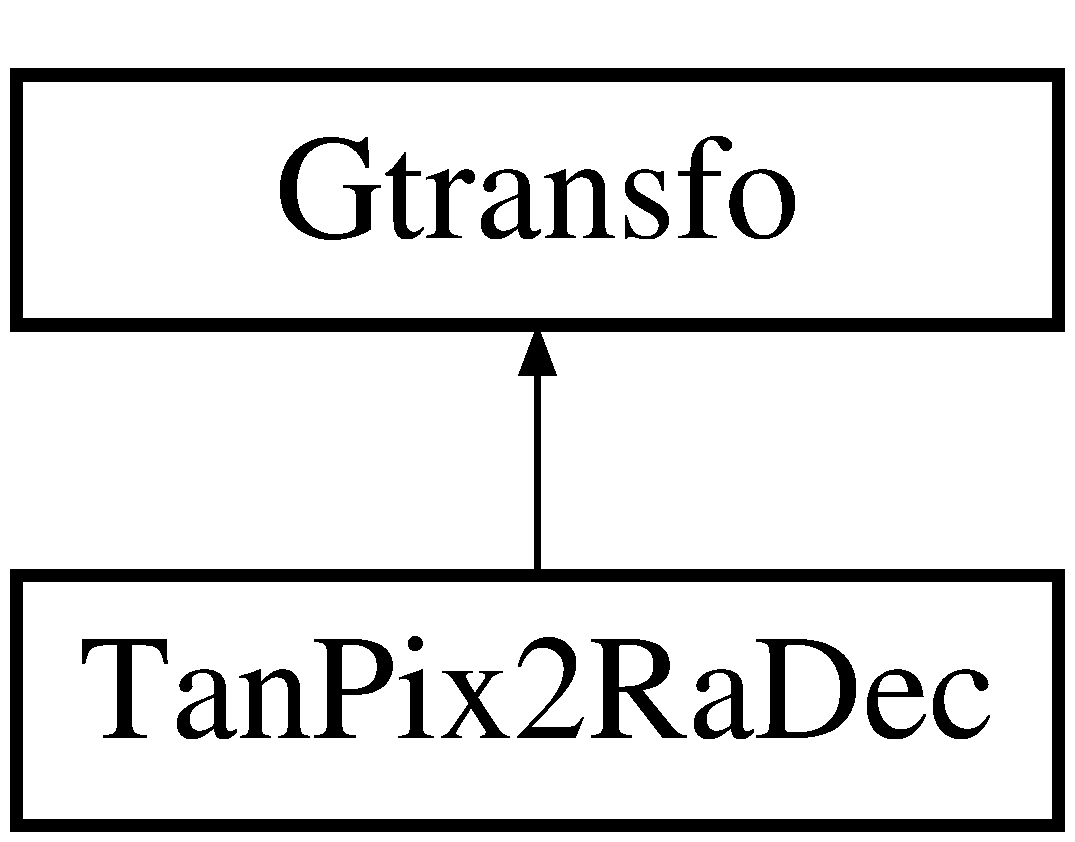
\includegraphics[height=2cm]{class_tanpix2radec}
\end{center}
\end{figure}
\subsubsection*{Public Methods}
\begin{CompactItemize}
\item 
\index{TanPix2RaDec@{TanPix2RaDec}!TanPix2RaDec@{Tan\-Pix2Ra\-Dec}}\index{TanPix2RaDec@{TanPix2RaDec}!TanPix2RaDec@{Tan\-Pix2Ra\-Dec}}
{\bf Tan\-Pix2Ra\-Dec} (const {\bf Gtransfo\-Lin} \&Pix2Tan, const {\bf Point} \&Tangent\-Point, const {\bf Gtransfo\-Quad} $\ast$Corrections=NULL)\label{class_tanpix2radec_a0}

\begin{CompactList}\small\item\em Pix2Tan describes the transfo from pix to tangent plane (in degrees). Tangent\-Point in degrees. Corrections are applied between Lin and deprojection parts (as in Swarp).\item\end{CompactList}\item 
\index{TanPix2RaDec@{TanPix2RaDec}!TanPix2RaDec@{Tan\-Pix2Ra\-Dec}}\index{TanPix2RaDec@{TanPix2RaDec}!TanPix2RaDec@{Tan\-Pix2Ra\-Dec}}
{\bf Tan\-Pix2Ra\-Dec} (const Tan\-Pix2Ra\-Dec \&Original)\label{class_tanpix2radec_a1}

\item 
\index{operator=@{operator=}!TanPix2RaDec@{Tan\-Pix2Ra\-Dec}}\index{TanPix2RaDec@{TanPix2RaDec}!operator=@{operator=}}
void {\bf operator=} (const Tan\-Pix2Ra\-Dec \&)\label{class_tanpix2radec_a2}

\item 
\index{TanPix2RaDec@{TanPix2RaDec}!TanPix2RaDec@{Tan\-Pix2Ra\-Dec}}\index{TanPix2RaDec@{TanPix2RaDec}!TanPix2RaDec@{Tan\-Pix2Ra\-Dec}}
{\bf Tan\-Pix2Ra\-Dec} ()\label{class_tanpix2radec_a3}

\item 
\index{apply@{apply}!TanPix2RaDec@{Tan\-Pix2Ra\-Dec}}\index{TanPix2RaDec@{TanPix2RaDec}!apply@{apply}}
void {\bf apply} (const double Xin, const double Yin, double \&Xout, double \&Yout) const\label{class_tanpix2radec_a4}

\item 
\index{apply@{apply}!TanPix2RaDec@{Tan\-Pix2Ra\-Dec}}\index{TanPix2RaDec@{TanPix2RaDec}!apply@{apply}}
{\bf Point} {\bf apply} (const {\bf Point} \&Pin) const\label{class_tanpix2radec_a5}

\item 
\index{operator *@{operator $\ast$}!TanPix2RaDec@{Tan\-Pix2Ra\-Dec}}\index{TanPix2RaDec@{TanPix2RaDec}!operator *@{operator $\ast$}}
Tan\-Pix2Ra\-Dec {\bf operator $\ast$} (const {\bf Gtransfo\-Lin} \&Right)\label{class_tanpix2radec_a6}

\begin{CompactList}\small\item\em composition with {\bf Gtransfo\-Lin} {\rm (p.\,\pageref{class_gtransfolin})}.\item\end{CompactList}\item 
\index{invert@{invert}!TanPix2RaDec@{Tan\-Pix2Ra\-Dec}}\index{TanPix2RaDec@{TanPix2RaDec}!invert@{invert}}
{\bf Tan\-Ra\-Dec2Pix} {\bf invert} () const\label{class_tanpix2radec_a7}

\begin{CompactList}\small\item\em approximate inverse : it ignores corrections;.\item\end{CompactList}\item 
\index{RoughInverse@{RoughInverse}!TanPix2RaDec@{Tan\-Pix2Ra\-Dec}}\index{TanPix2RaDec@{TanPix2RaDec}!RoughInverse@{Rough\-Inverse}}
{\bf Gtransfo}$\ast$ {\bf Rough\-Inverse} (const {\bf Frame} \&Region) const\label{class_tanpix2radec_a8}

\begin{CompactList}\small\item\em Overload the \char`\"{}generic routine\char`\"{} (available for all {\bf Gtransfo} {\rm (p.\,\pageref{class_gtransfo})} types.\item\end{CompactList}\item 
\index{InverseTransfo@{InverseTransfo}!TanPix2RaDec@{Tan\-Pix2Ra\-Dec}}\index{TanPix2RaDec@{TanPix2RaDec}!InverseTransfo@{Inverse\-Transfo}}
{\bf Gtransfo}$\ast$ {\bf Inverse\-Transfo} (const double Precision, const {\bf Frame} \&Region) const\label{class_tanpix2radec_a9}

\begin{CompactList}\small\item\em Inverse transfo: returns a {\bf Tan\-Ra\-Dec2Pix} {\rm (p.\,\pageref{class_tanradec2pix})} if there are no corrections, or the iterative solver if there are.\item\end{CompactList}\item 
\index{SetCorrections@{SetCorrections}!TanPix2RaDec@{Tan\-Pix2Ra\-Dec}}\index{TanPix2RaDec@{TanPix2RaDec}!SetCorrections@{Set\-Corrections}}
void {\bf Set\-Corrections} (const {\bf Gtransfo\-Quad} $\ast$Corrections)\label{class_tanpix2radec_a10}

\begin{CompactList}\small\item\em Sets the corrections (it can be a cubic ocrrection).\item\end{CompactList}\item 
\index{Clone@{Clone}!TanPix2RaDec@{Tan\-Pix2Ra\-Dec}}\index{TanPix2RaDec@{TanPix2RaDec}!Clone@{Clone}}
{\bf Gtransfo}$\ast$ {\bf Clone} () const\label{class_tanpix2radec_a11}

\begin{CompactList}\small\item\em returns a copy (allocated by new) of the transformation.\item\end{CompactList}\item 
\index{dump@{dump}!TanPix2RaDec@{Tan\-Pix2Ra\-Dec}}\index{TanPix2RaDec@{TanPix2RaDec}!dump@{dump}}
void {\bf dump} (ostream \&stream) const\label{class_tanpix2radec_a12}

\begin{CompactList}\small\item\em dumps the transfo coefficients to stream.\item\end{CompactList}\item 
\index{TangentPoint@{TangentPoint}!TanPix2RaDec@{Tan\-Pix2Ra\-Dec}}\index{TanPix2RaDec@{TanPix2RaDec}!TangentPoint@{Tangent\-Point}}
{\bf Point} {\bf Tangent\-Point} () const\label{class_tanpix2radec_a13}

\begin{CompactList}\small\item\em The tangent point (in degrees).\item\end{CompactList}\item 
\index{LinPart@{LinPart}!TanPix2RaDec@{Tan\-Pix2Ra\-Dec}}\index{TanPix2RaDec@{TanPix2RaDec}!LinPart@{Lin\-Part}}
{\bf Gtransfo\-Lin} {\bf Lin\-Part} () const\label{class_tanpix2radec_a14}

\begin{CompactList}\small\item\em The Linear part (corresponding to CD's and CRPIX's).\item\end{CompactList}\item 
\index{Corr@{Corr}!TanPix2RaDec@{Tan\-Pix2Ra\-Dec}}\index{TanPix2RaDec@{TanPix2RaDec}!Corr@{Corr}}
const {\bf Gtransfo\-Quad}$\ast$ {\bf Corr} () const\label{class_tanpix2radec_a15}

\begin{CompactList}\small\item\em the correction (can be more than quadratic).\item\end{CompactList}\item 
\index{CrPix@{CrPix}!TanPix2RaDec@{Tan\-Pix2Ra\-Dec}}\index{TanPix2RaDec@{TanPix2RaDec}!CrPix@{Cr\-Pix}}
{\bf Point} {\bf Cr\-Pix} () const\label{class_tanpix2radec_a16}

\begin{CompactList}\small\item\em the CRPIX values (this is WCS jargon).\item\end{CompactList}\item 
double {\bf fit} (const Star\-Match\-List \&List, const {\bf Gtransfo} $\ast$Prior\-Transfo=NULL, const {\bf Gtransfo} $\ast$Posterior\-Transfo=NULL)
\begin{CompactList}\small\item\em fits a transfo to a list of star pairs (p1,p2).\item\end{CompactList}\item 
\index{~TanPix2RaDec@{$\sim$TanPix2RaDec}!TanPix2RaDec@{Tan\-Pix2Ra\-Dec}}\index{TanPix2RaDec@{TanPix2RaDec}!~TanPix2RaDec@{$\sim$Tan\-Pix2Ra\-Dec}}
{\bf $\sim$Tan\-Pix2Ra\-Dec} ()\label{class_tanpix2radec_a18}

\end{CompactItemize}


\subsubsection{Detailed Description}
the transformation that handles pix to sideral transfos (Gnomonic, possibly with polynomial distortions).



\subsubsection{Member Function Documentation}
\index{TanPix2RaDec@{Tan\-Pix2Ra\-Dec}!fit@{fit}}
\index{fit@{fit}!TanPix2RaDec@{Tan\-Pix2Ra\-Dec}}
\paragraph{\setlength{\rightskip}{0pt plus 5cm}double Tan\-Pix2Ra\-Dec::fit (const Star\-Match\-List \& {\em List}, const {\bf Gtransfo} $\ast$ {\em Prior\-Transfo} = NULL, const {\bf Gtransfo} $\ast$ {\em Posterior\-Transfo} = NULL)\hspace{0.3cm}{\tt  [virtual]}}\hfill\label{class_tanpix2radec_a17}


fits a transfo to a list of star pairs (p1,p2).

After the fit this(Prior\-Transfo(p1)) yields approximately Posterior\-Transfo(p2). The returned value is the chi2. 

Reimplemented from {\bf Gtransfo} {\rm (p.\,\pageref{class_gtransfo_a4})}.

The documentation for this class was generated from the following file:\begin{CompactItemize}
\item 
{\bf gtransfo.h}\end{CompactItemize}
